\documentclass{article}

\usepackage{geometry}
\usepackage{amsmath}
\usepackage{graphicx, eso-pic}
\usepackage{listings}
\usepackage{hyperref}
\usepackage{multicol}
\usepackage{fancyhdr}
\pagestyle{fancy}
\fancyhf{}
\hypersetup{ colorlinks=true, linkcolor=black, filecolor=magenta, urlcolor=cyan}
\geometry{ a4paper, total={170mm,257mm}, top=40mm, right=20mm, bottom=20mm, left=20mm}
\setlength{\parindent}{0pt}
\setlength{\parskip}{0.3em}
\renewcommand{\headrulewidth}{0pt}
\AddToShipoutPictureBG{%
  \AtPageUpperLeft{%
    \raisebox{-\height}{
\includegraphics[width=\paperwidth, height=30mm]{../headerarkav.png}}
  }
}
\rfoot{\thepage}
\lfoot{Penyisihan Competitive Programming - Arkavidia 7.0}
\lstset{
    basicstyle=\ttfamily\small,
    columns=fixed,
    extendedchars=true,
    breaklines=true,
    tabsize=2,
    prebreak=\raisebox{0ex}[0ex][0ex]{\ensuremath{\hookleftarrow}},
    frame=none,
    showtabs=false,
    showspaces=false,
    showstringspaces=false,
    prebreak={},
    keywordstyle=\color[rgb]{0.627,0.126,0.941},
    commentstyle=\color[rgb]{0.133,0.545,0.133},
    stringstyle=\color[rgb]{01,0,0},
    captionpos=t,
    escapeinside={(\%}{\%)}
}

\begin{document}

\begin{center}
    \section*{J - Jumlah Opat} % ganti judul soal

    \begin{tabular}{ | c c | }
        \hline
        Batas Waktu  & 2s \\    % jangan lupa ganti time limit
        Batas Memori & 256MB \\  % jangan lupa ganti memory limit
        \hline
    \end{tabular}
\end{center}

\subsection*{Deskripsi}
Diberikan \textbf{forest} dengan $N$ buah \textit{node} dan $M$ buah \textit{edge}. \textit{Node} dengan indeks ke-$i$ memiliki nilai $A_i$.

Carilah sebuah \textbf{connected subgraph} dengan minimal $2$ \textit{node} dari \textbf{forest} tersebut yang jumlah nilainya habis dibagi $4$. 

Apabila terdapat banyak solusi, keluarkan yang mana saja.

Apabila tidak terdapat solusi, keluarkan -1.

\textbf{Catatan:} 
\begin{itemize}
    \setlength\itemsep{0pt}
    \item Sebuah \textbf{forest} merupakan kumpulan \textit{tree} atau \textit{graph} asiklik yang tidak harus \textit{connected} atau terhubung. 
    \item Suatu \textbf{connected subgraph} merupakan \textbf{connected graph} yang didapatkan dengan penghapusan beberapa \textit{node} dan/atau \textit{edge} dari \textit{graph} asal.
\end{itemize}

\subsection*{Format Masukan}

Baris pertama terdiri dari dua buah integer $N$ $(3 \leq N \leq 3\times10^{5})$ dan $M$ $(0 \leq M \leq N-1)$, masing-masing menyatakan banyak \textit{node} dan banyak \textit{edge} dari suatu \textbf{forest}.
\\\\
Baris kedua terdiri dari $N$ buah integer $A_1,A_2,...,A_N$ $(0 \leq A_i \leq 10^9)$ yang menyatakan nilai dari \textit{node} suatu \textbf{forest}.
\\\\
$M$ baris selanjutnya berisi sepasang integer $U$ dan $V$ yang menyatakan \textit{edge} dari suatu \textbf{forest} di mana $U$ dan $V$ masing-masing merupakan \textit{indeks} \textit{node} \textbf{forest} tersebut.


\subsection*{Format Keluaran}
Jika terdapat solusi, keluaran terdiri dari $2$ baris.

Baris pertama terdiri dari sebuah integer $K$, yang menyatakan banyak \textit{node} dari \textbf{connected subgraph} yang memenuhi.

Baris kedua terdiri dari $K$ buah integer $U_1,U_2,...,U_k$ yang menyatakan \textbf{indeks} \textit{node} dari \textbf{connected subgraph} yang memenuhi.

Jika terdapat lebih dari $1$ buah solusi, keluarkan yang mana saja. 

Jika tidak terdapat solusi, cukup keluarkan $-1$.
\pagebreak
\begin{multicols}{2}
\subsection*{Contoh Masukan 1}
\begin{lstlisting}
8 7
1 2 3 4 5 6 7 8
1 2
1 4
1 8
2 3
2 5
4 6
4 7
\end{lstlisting}
\columnbreak
\subsection*{Contoh Keluaran 1}
\begin{lstlisting}
5
3 1 2 6 4
\end{lstlisting}
\vfill
\null
\end{multicols}

\begin{multicols}{2}
\subsection*{Contoh Masukan 2}
\begin{lstlisting}
6 4
2 3 2 2 2 2
1 2
2 3
2 4
2 6
\end{lstlisting}
\columnbreak
\subsection*{Contoh Keluaran 2}
\begin{lstlisting}
-1
\end{lstlisting}
\vfill
\null
\end{multicols}

\subsection*{Penjelasan}
Pada \textit{test case} pertama, kita dapat gambarkan graph sebagai berikut:
\begin{center}
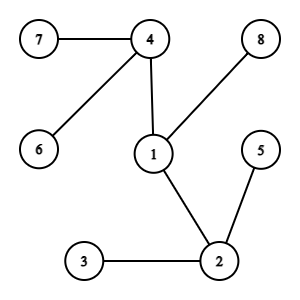
\includegraphics[scale=0.5]{tc1.png}
\end{center}
\textit{node-node} ${3,1,2,6,4}$ membentuk sebuah \textbf{connected subgraph} pada \textbf{forest} masukan yang memiliki jumlah nilai $16$ dan lebih dari $1$ \textit{node}. \\

Pada \textit{test case} kedua, tidak ada \textbf{connected subgraph} pada \textbf{forest} masukan yang memiliki jumlah nilai yang habis dibagi 4.

\end{document}